\subsection{Background}
The previous year decided to create a new design of the Aerodynamics Test Platform (ATP) from scratch. They preformed various computer simulations including Finite Element Analysis (FEA) for manufactured components and testing of various designs within MSC Adams to determine which would be the most stable under the oscillations induced by the flapper. Below is an image of the final ATP design CAD model.

\begin{figure}[htb]
  \centering
  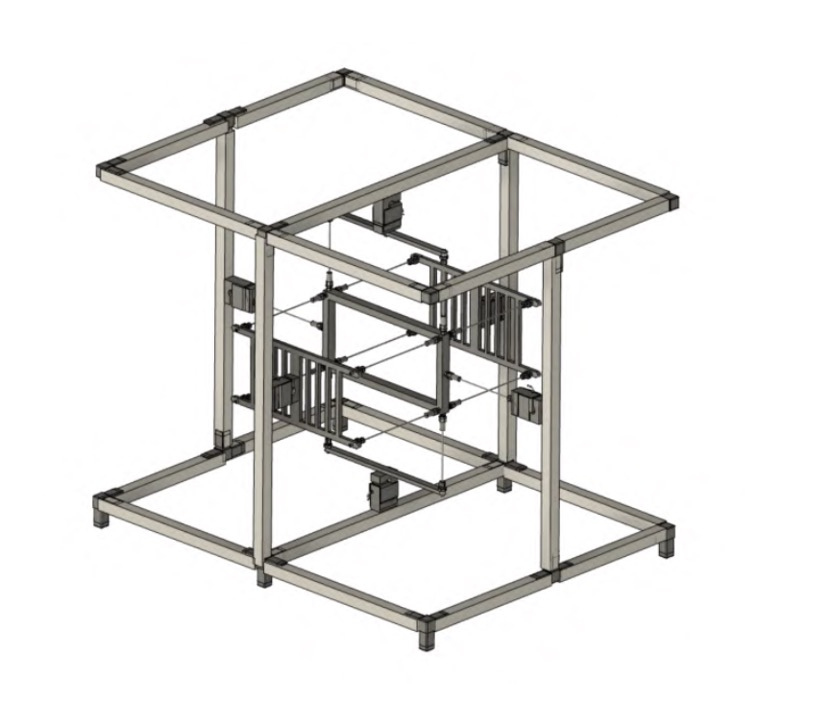
\includegraphics[height=6.5cm]{figures/Previous Year's ATP Design.jpg}
  \caption{Previous Year's ATP Design.}
  \label{fig:Previous_ATP_Design}
\end{figure}

The design consists of an outer frame made from aluminum extrusion and plastic press fit connectors. The base of the load cells are secured to the outer frame, the active end of the load cells are connected to crossbars using barrel adjusters and eight inch steel cables. There are six load cells within the design, two in each axis of motion. The crossbars are connected to the inner frame using more barrel adjusters and eight inch steel cables.

The previous year's team completed this design and was able to assemble the outer frame and some of the crossbars and cables. However, due to shipping timelines they were unable to assemble the entire design and begin testing.

In their handover letter, the previous year's team recommended the design of the inner frame be re-evaluated to better integrate with the flapper as well as the steel wire attachment mechanism between the inner frame and crossbars.

\subsection{Taking Stock of the Previous ATP Design}

The semester began by reviewing the previous year's progress on the ATP, and getting my hands on the ATP. Below is an image of the state of the ATP at the start of the year.

\begin{figure}[htb]
  \centering
  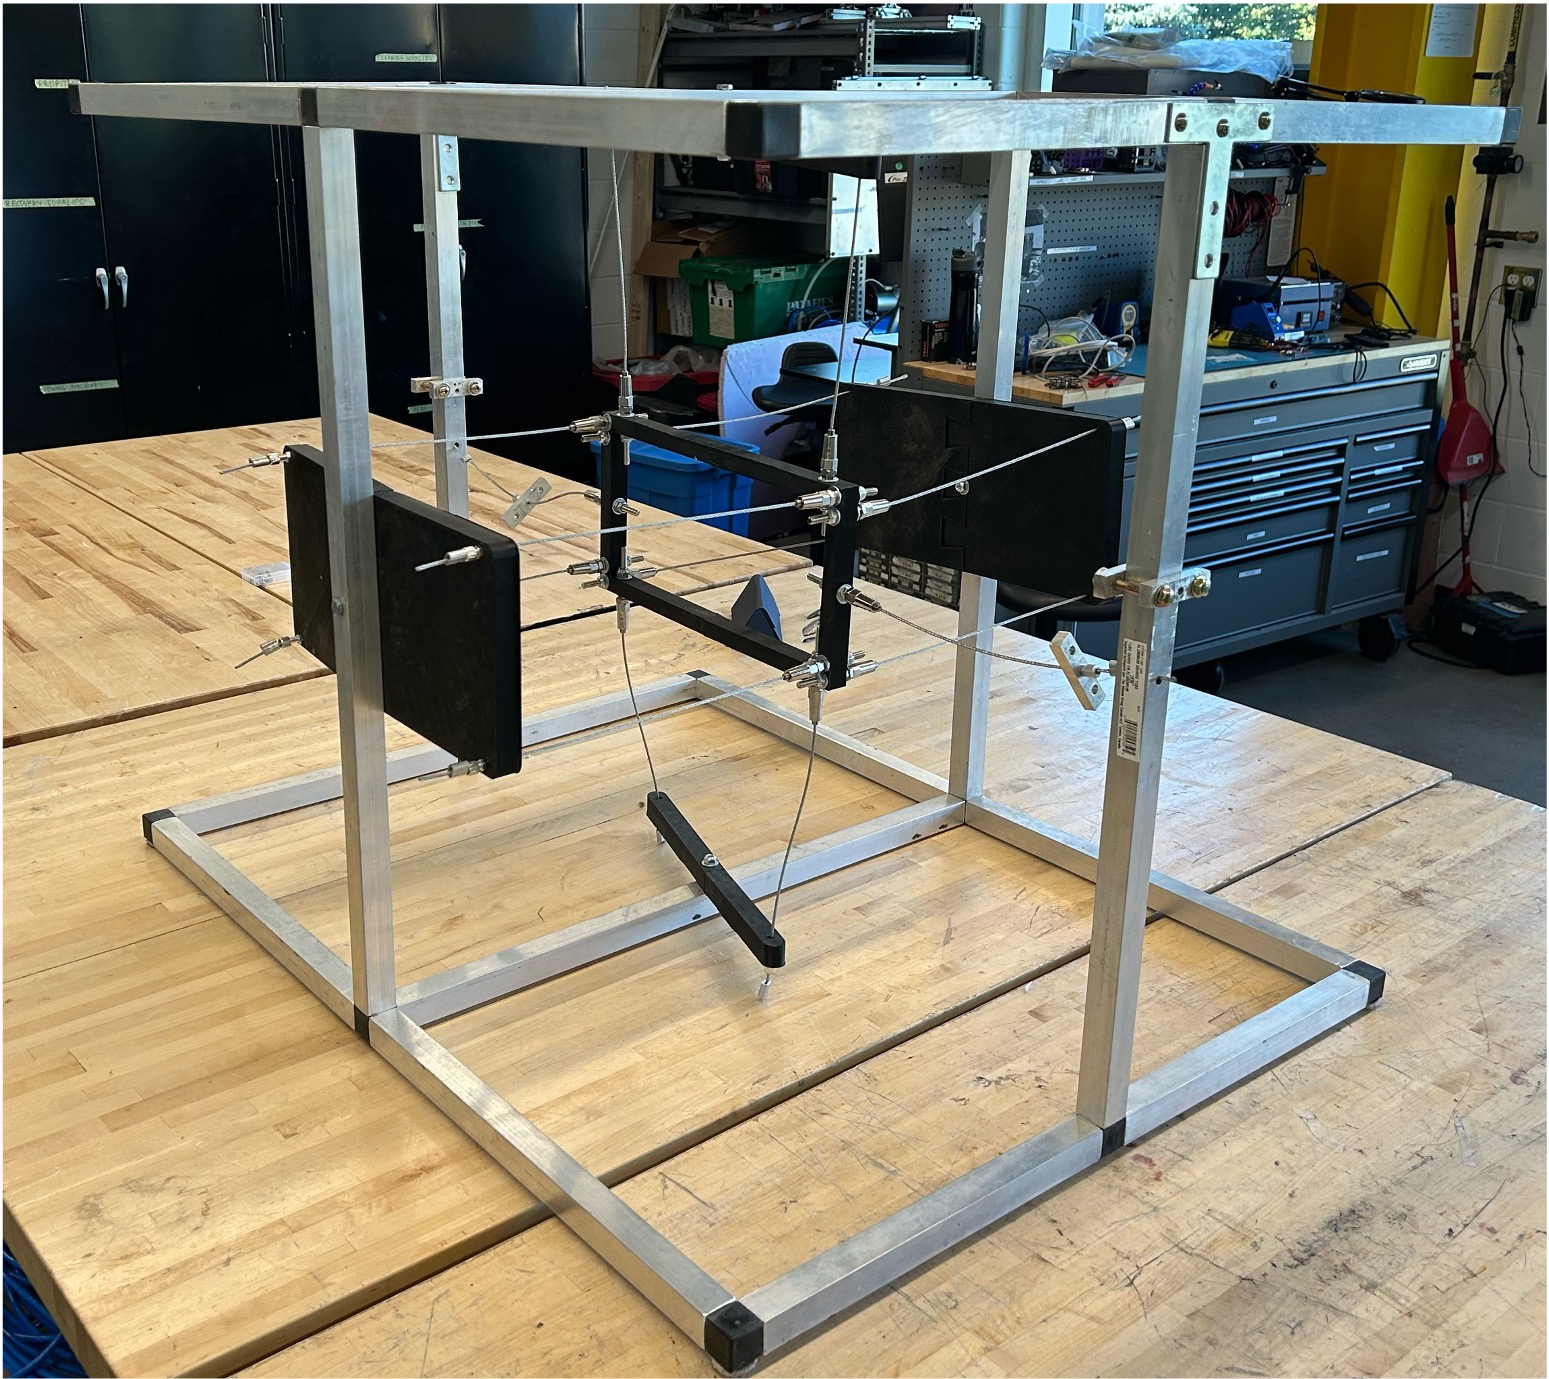
\includegraphics[height=6.5cm]{figures/State of ATP Sep 2025.jpg}
  \caption{State of the ATP at the beginning of the Fall Semester.}
  \label{fig:State_Of_ATP_Sep}
\end{figure}

Looking at Figure \ref{fig:State_Of_ATP_Sep}, we see the aluminum outer frame, 3D printed inner frame and crossbars, as well as the steel cables connecting some of the components together. During my inspections of the ATP I noticed many of the 3D printed components were prototype components and were printed in multiple pieces and glued together afterwards, creating large variations in accuracy and built quality. Additionally, I observed the barrel adjusters did not offer much adjustment for the tensioning of the steel cables, being able to tension these cables would be necessary once the time came to integrate the load cells into the ATP. Based off the recommendations of the previous year's team and my own observation I decided a re-design of the inner frame and attachment mechanism was in order.

I began by creating a CAD model of the outer frame based off the dimensions of the assembled ATP. With the outer frame accurately modelled, I could turn my attention to taking stock of the components we had on hand. I partially disassembled the ATP by removing all 3D printed components, steel cables, and couplings from the ATP. I recorded the part numbers of the couplings and measured the distances of the steel cables for later reference during the design process. Once this was complete, I was left with a bare outer frame.

\subsection{Re-Designing the Inner Frame and Couplings}

My next step was to re-design the inner frame as well as the coupling mechanism. Over the course of several weeks of iteration and design reviews with professor Garcias, I came up with a redesign of both the inner frame and coupling mechanism. 

\begin{figure}[htb]
  \centering
  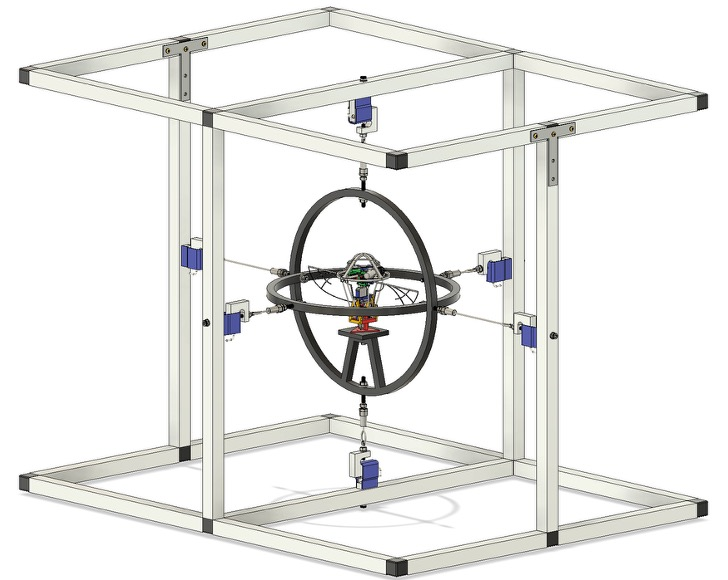
\includegraphics[height=6.5cm]{figures/Completed ATP Design.jpg}
  \caption{CAD Model of the current ATP Design.}
  \label{fig:Current_ATP_Design}
\end{figure}

The inner frame consists of two concentric 3D printed rings in addition to a 3D printed adapter plate to which the flapper can be mounted, the updated inner frame design can be seen in Figure \ref{fig:Current_ATP_Design}. As for the coupling mechanism, one side utilizes the existing stud couplers from the previous design to bolt through the inner frame. To attach the other end to the load cells, M6 stud anchors were used in conjunction with an M6 washer and nut, the steel cable could then be thread through the eyelet of the stud anchor and crimped back on itself. See Figures \ref{fig:Coupling_Mechanism} and \ref{fig:Coupling_Mechanism_Cross_Section} for a close-up view of the attachment mechanism. This attachment mechanism allowed for a large range of adjustment during the assembly process to control the tensions within the steel cables with a high degree of accuracy.

\begin{figure}
\centering
\begin{subfigure}{.5\textwidth}
  \centering
  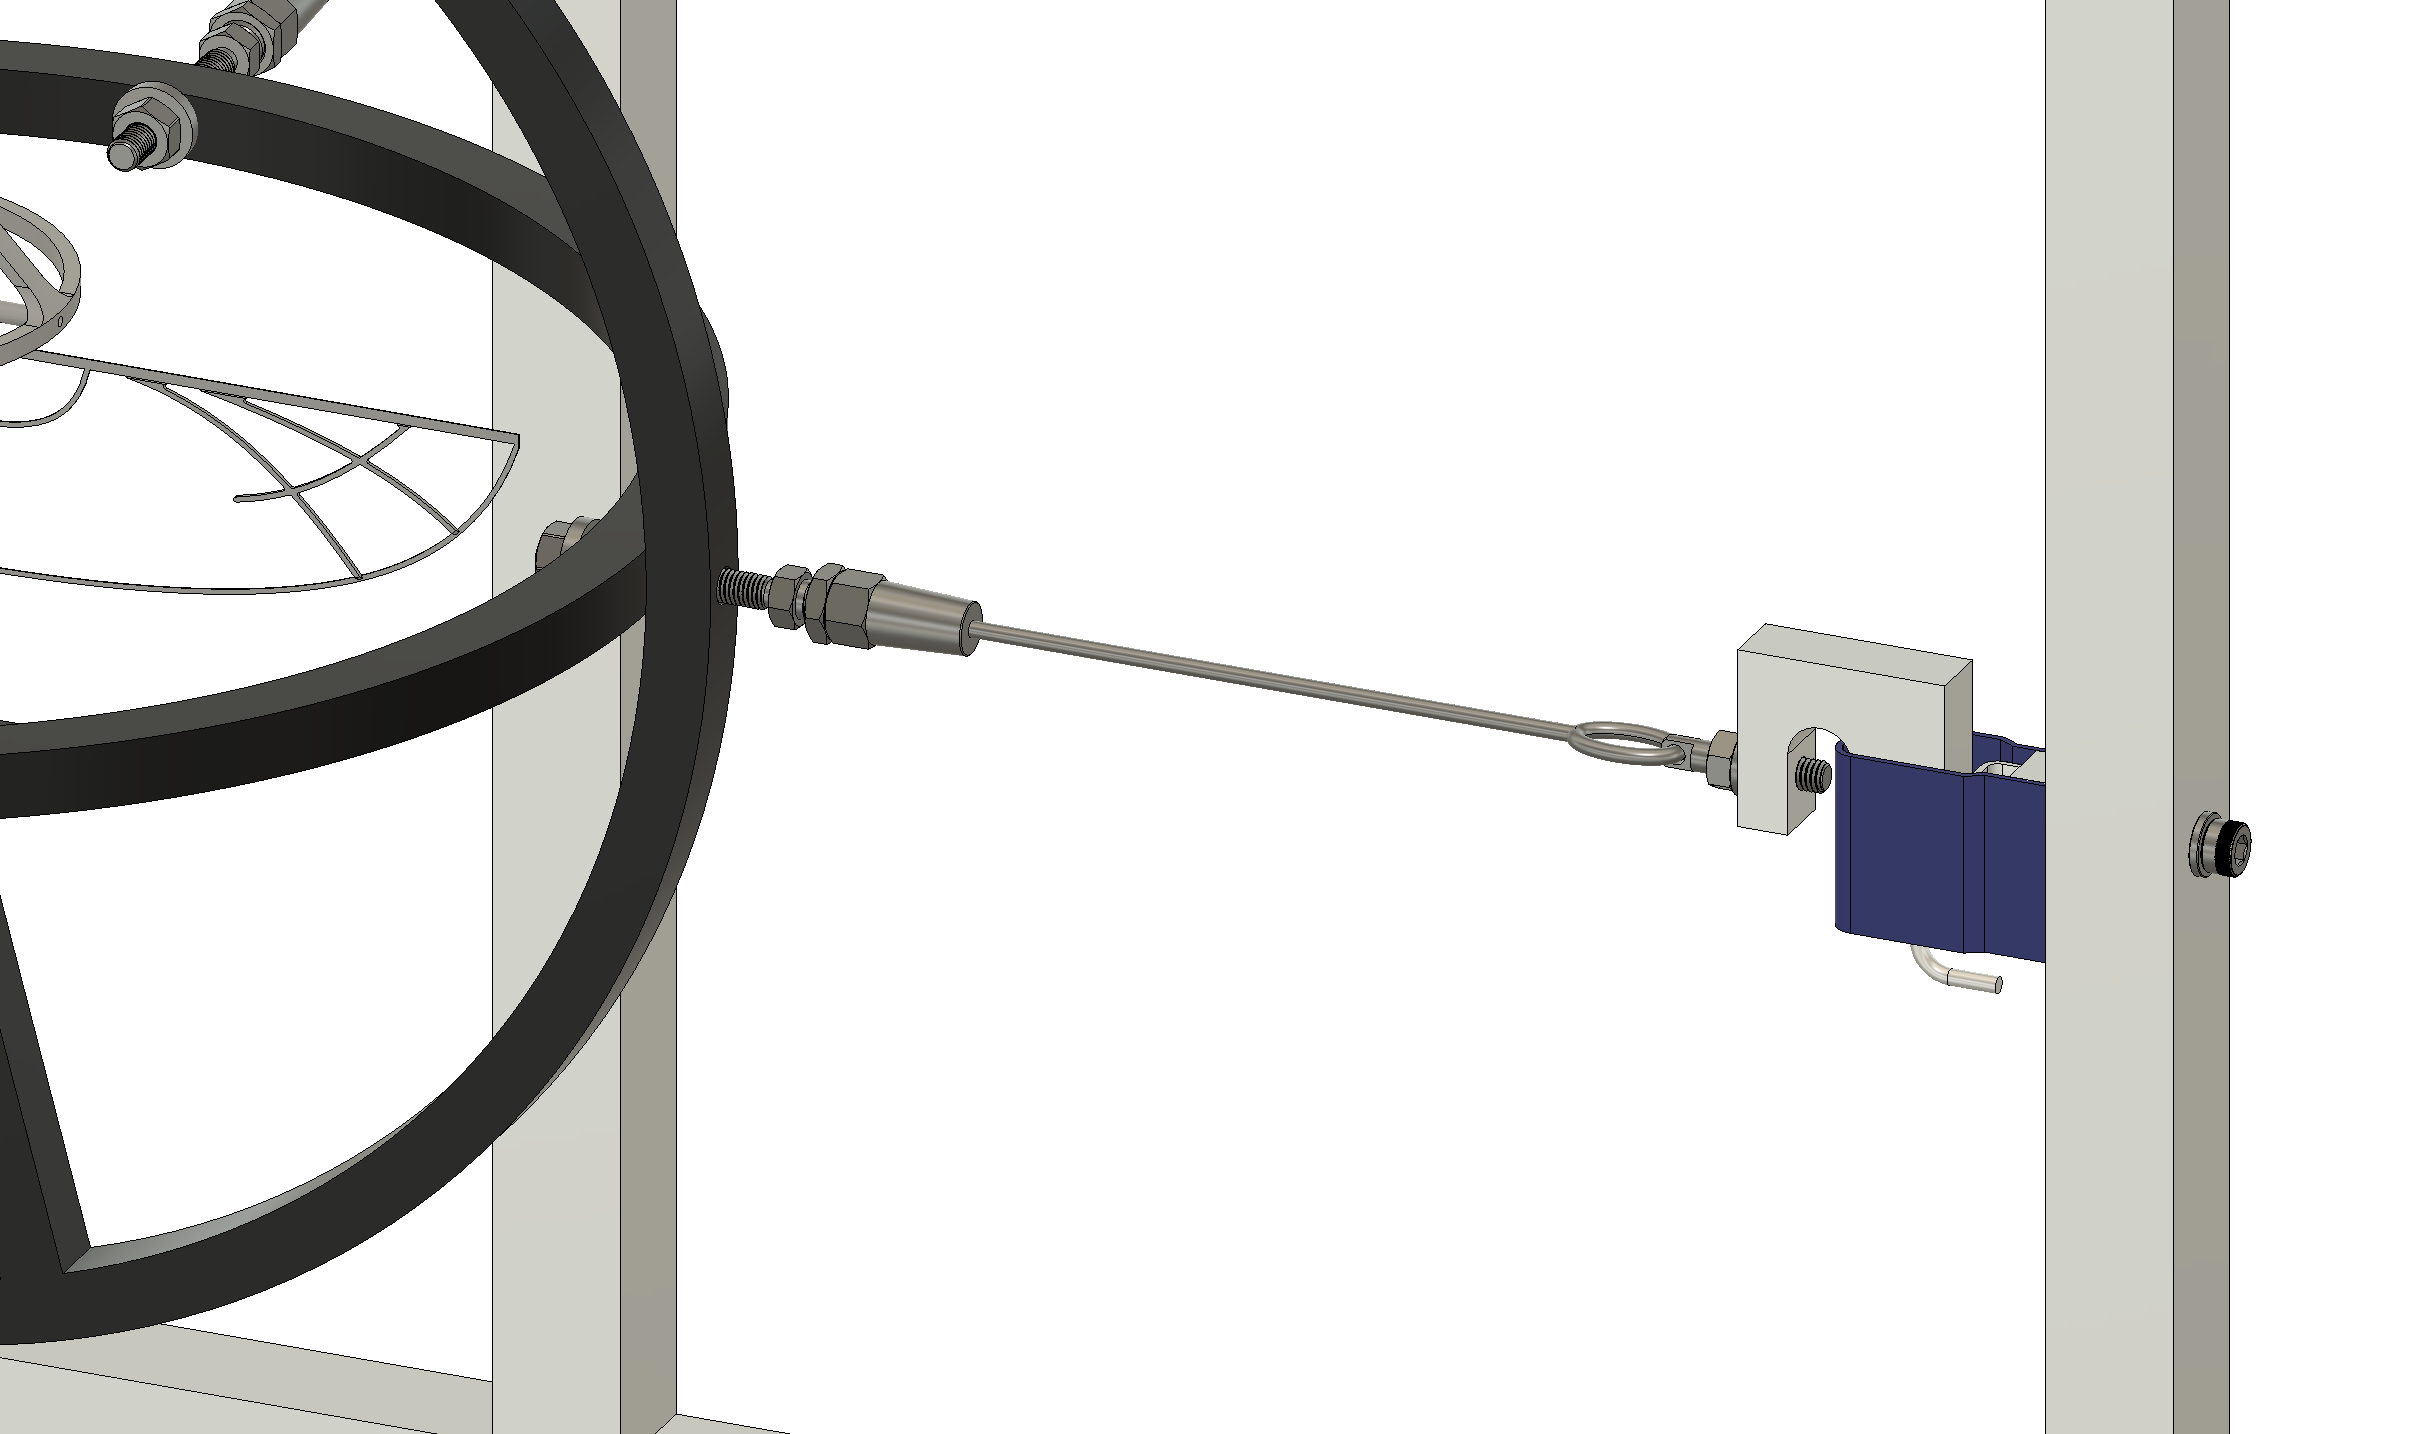
\includegraphics[height=4.5cm]{figures/Coupling Close Up.png}
  \caption{Close-Up of the Coupling Mechanism.}
  \label{fig:Coupling_Mechanism}
\end{subfigure}%
\begin{subfigure}{.5\textwidth}
  \centering
  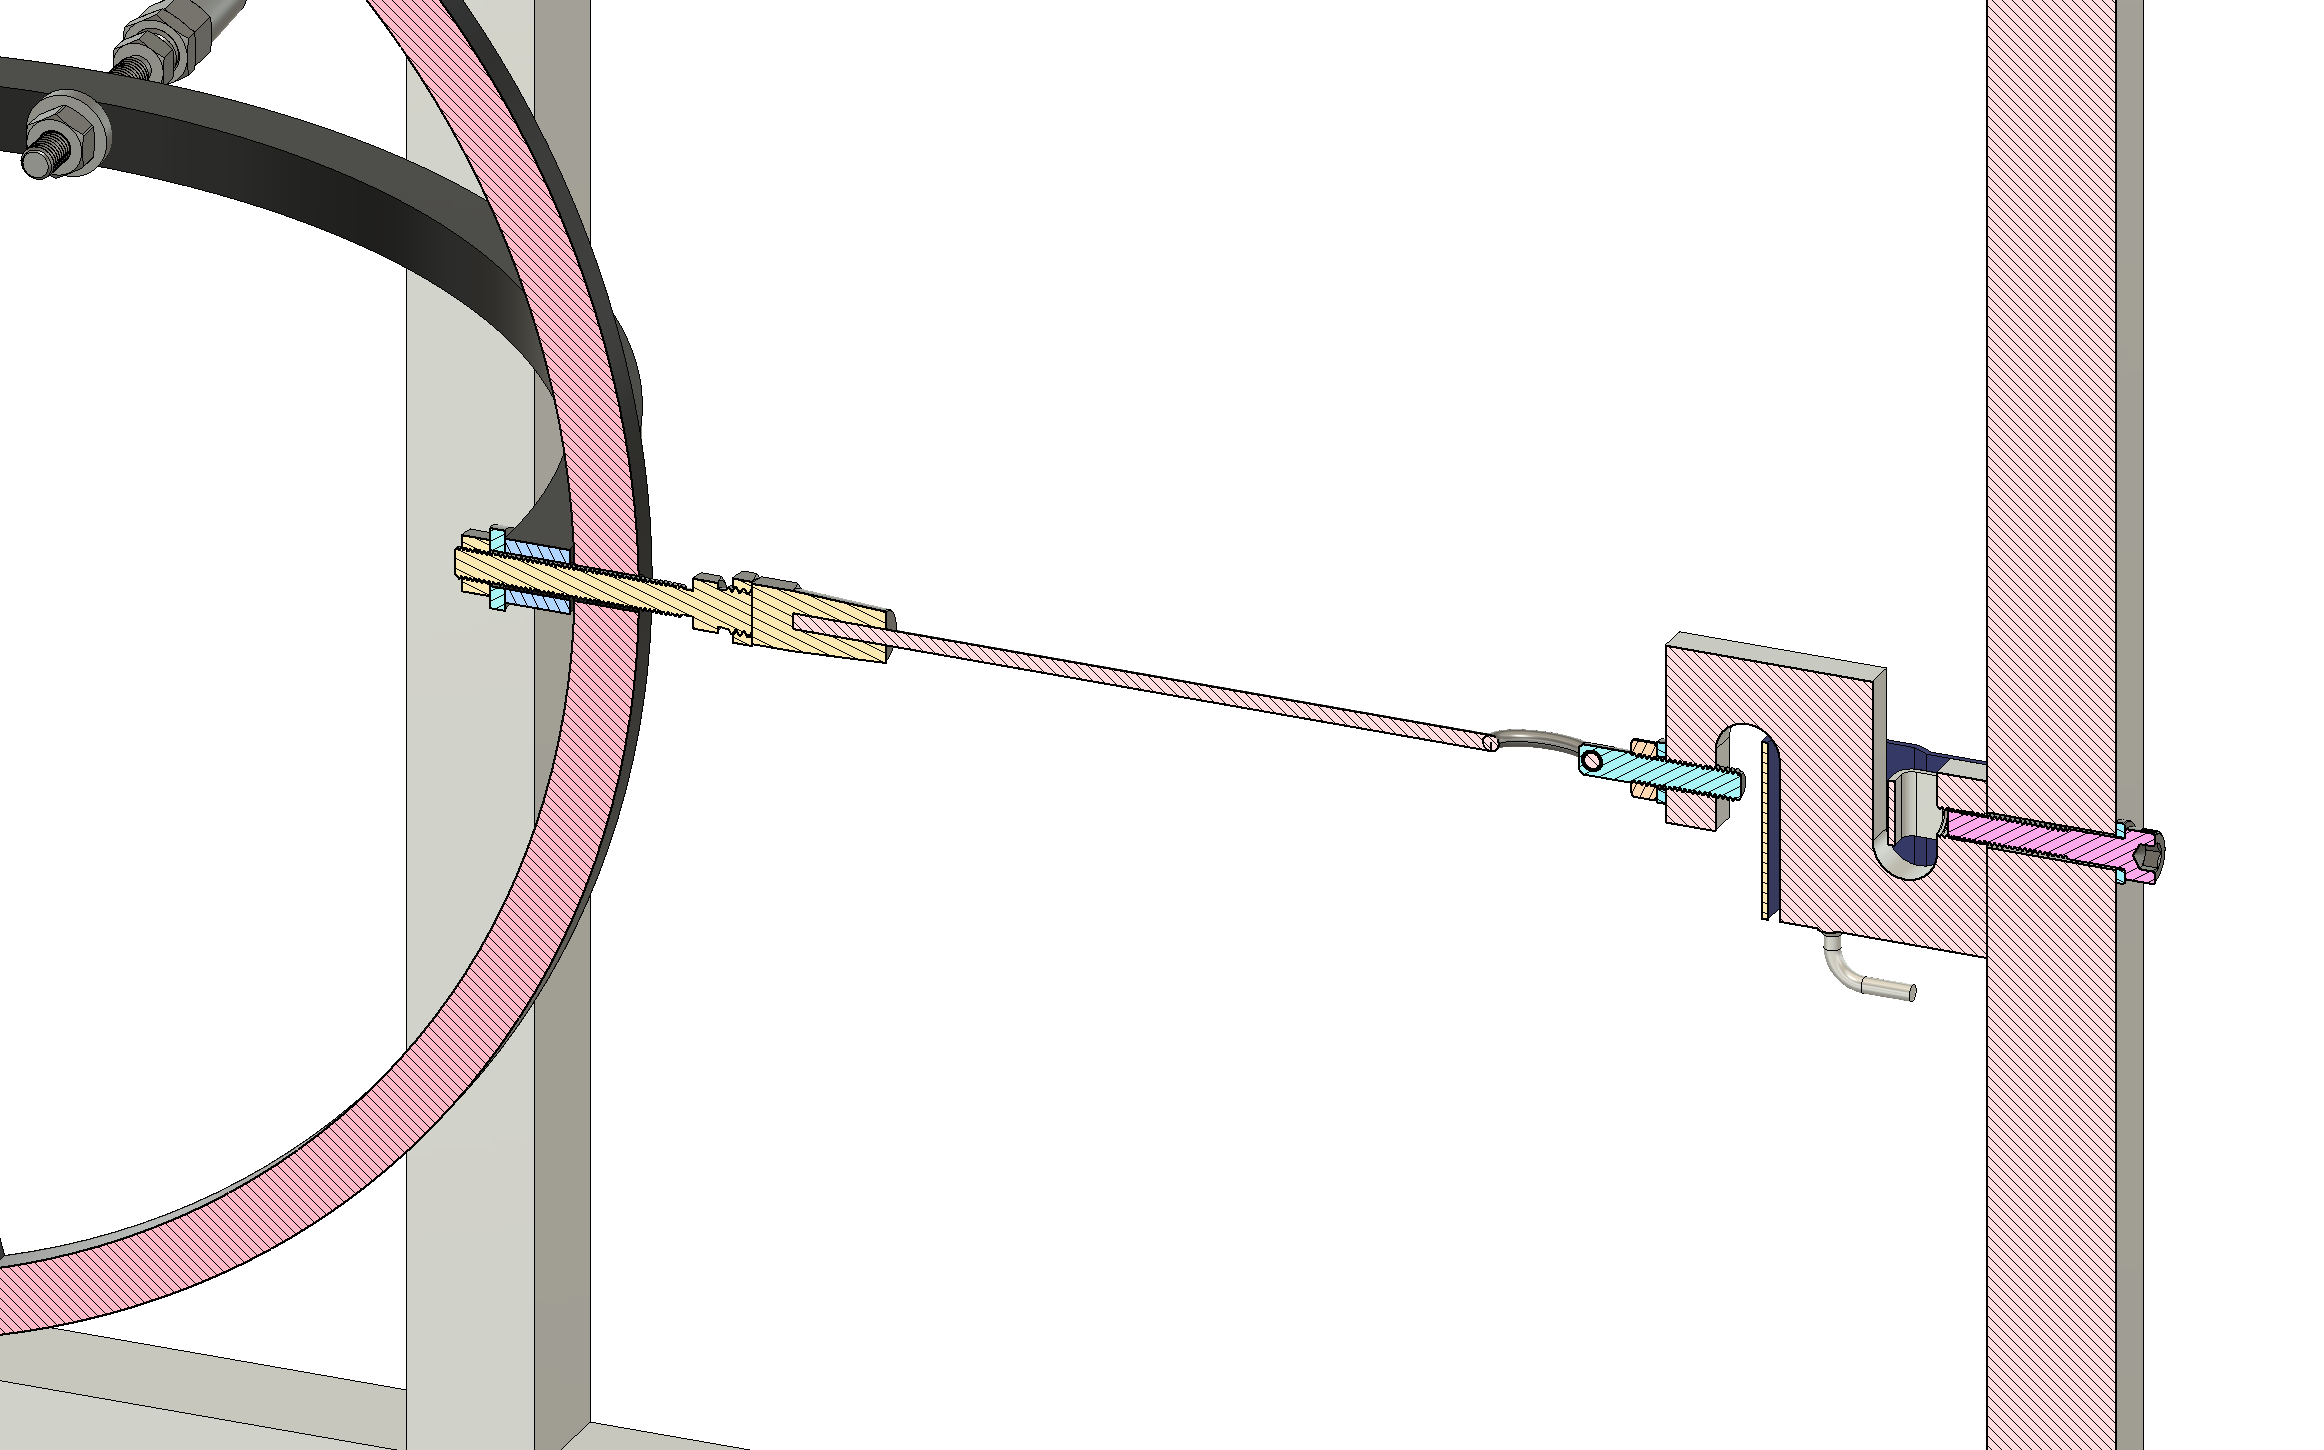
\includegraphics[height=4.5cm]{figures/Coupling Close Up Cross Section.png}
  \caption{\label{fig:right_robot} Cross Section of the Coupling Mechanism.}
  \label{fig:Coupling_Mechanism_Cross_Section}
\end{subfigure}
\caption{Detailed Views of the Coupling Mechanism.}
\label{fig:test}
\end{figure}

\subsection{Assembly and Testing}
With the design complete, it was now time to manufacture, assemble, and begin testing. The manufacturing was minimal and fast by design, only three components required manufacturing; the two 3D printed inner rings and the 3D printed adapter plate. In the meantime, the required components could be ordered from McMaster Carr. The required components consisted of mainly fasteners with the exception of the M6 stud anchors, M6 standoffs (To be used in place of the load cells during storage and assembly.), and steel cable crimp connectors.

With all components on hand the ATP could then be assembled. Assembly consisted of installing the M6 standoffs in place of the load cells, followed by measuring, cutting, and crimping the steel cables to length with the stud anchors in place. Lastly, the stud couplers could be bolted through the 3D printed inner frame rings. See Figure \ref{fig:Assembled_ATP} for an image of the assembled ATP.

\begin{figure}[htb]
  \centering
  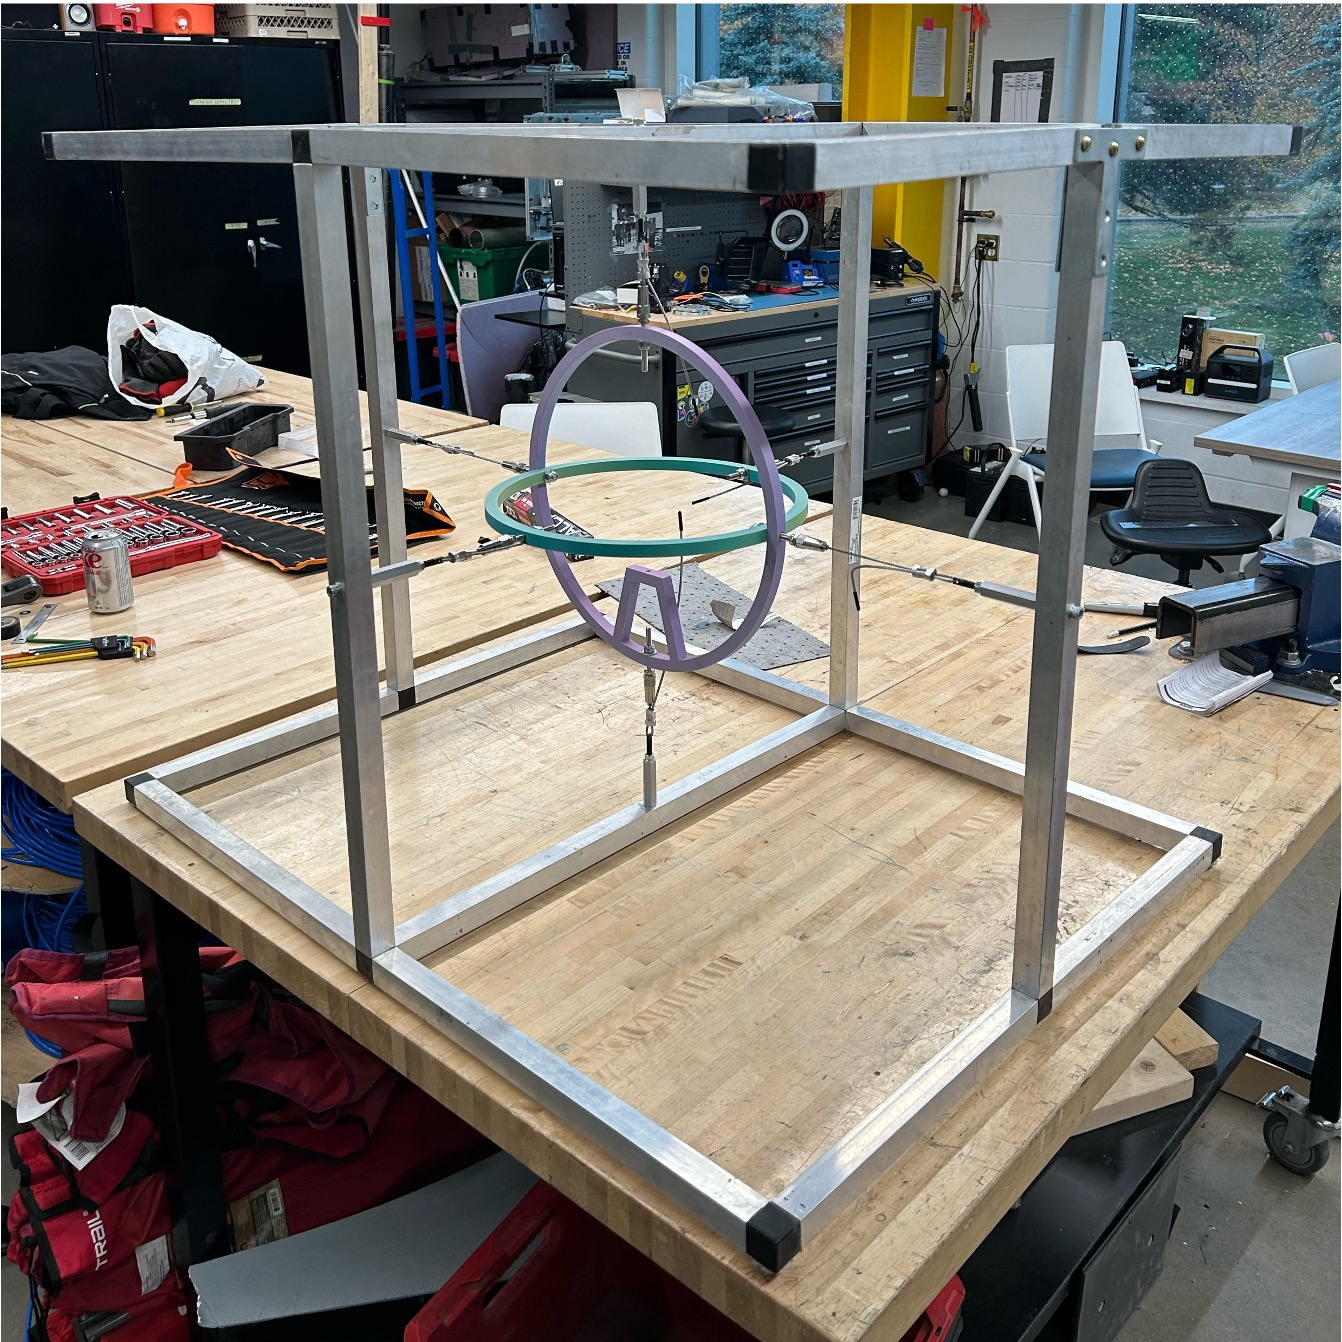
\includegraphics[height=6.5cm]{figures/Assembled ATP.jpg}
  \caption{Assembled ATP.}
  \label{fig:Assembled_ATP}
\end{figure}

With assembly complete, testing could begin. Testing is a joint effort with Kevin Fair as his role is Sensor Integration and Data Acquisition for the ATP. By this point in the semester, Kevin had gotten a single load cell functional with a laptop and LabVIEW to read the output voltage. We tested the load cell in both the horizontal and vertical orientations as well as various tensions for the steel cables. Our testing consisted of placing a series of decreasing masses onto the adapter plate and checking the output voltage of the load cell to determine the smallest detectable mass. During out initial tests, the smallest mass we detected was 200 grams. At a target flapper weight of 40 grams, this result was displeasing. Since this design utilizes steel cables, which work under tension, to achieve the desired rigidity these steel cables must be pre-tensioned. Our testing found that as this pre-tension force (And therefore the rigidity of the steel cables.) is increased, the resolution of our load cell decreased and vice-versa. Kevin talks in depth about this within section \ref{chap:Kevin_Fair} of this report. Kevin has since been able to mitigate this issue via voltage subtraction and other means discussed within his section.

With the results from our testing, my next step was to attempt to reduce the static mass of the design. With a lower static mass, the tensile forces required to support the design would be lower and therefore the resolution of the load cells could be increased.  I focused my efforts on the steel cables and couplings as these components were the heaviest. I sketched a 3D printed coupler which utilizes a bore and a tapered thread to clamp existing carbon fiber cable (Leftover from the previous year.) this coupler then connects to the thread of the load cell. This concluded my work for the fall semester.

\subsection{Plan for Winter Semester}
Moving into the winter semester, my overall goal is to get the ATP functional and able to collect data. This will primarily consist of testing and prototyping with Kevin throughout the semester.

As for the short term, I will turn my updated coupler concept into a function CAD design. I would like to design a method of adjusting the tension within the cables to help with assembly and prototyping. Once designed, manufacturing (3D printing) will occur, followed by assembly and testing. Testing will be similar to the testing process preformed previously, the load cell will be tested in a variety of orientations and analyzed using a variety of masses. Once we are satisfied with the testing results for a single load, the integration of the remaining five load cells will follow. Once all load cells our preforming as expected, data logging can begin.